\subsection{Definicje}
Definicje zostały zaczerpnięte z literatury, z pozycji \cite{Wilson2012}, \cite{Wloch2008} oraz \cite{Wojciechwoski2013}.

\noindent
\textbf{Definicja 1.}
Grafem nieskierowanym, skończonym G nazywamy parę $(V,E)$, gdzie $V = V(G)$ jest zbiorem skończonym, niepustym,
natomiast $E = E(V)$ jest rodziną mogących się powtarzać dwuelementowych podzbiorów niekoniecznie różnych elementów ze zbioru $V$.
Zbiór $V(G)$ nazywamy zbiorem wierzchołków (lub węzłami), a elementy tego zbioru nazywamy wierzchołkami i oznaczamy symbolami:
$x$, $y$, $x_i$, $y_i$, $1$, $2$, ... Zbiór $E(G)$ nazywamy zbiorem krawędzi grafu $G$.
Mówimy, że krawędź $\{v, w\}$ łączy wierzchołki $v$ i $w$, i na ogół oznaczamy ją krócej symbolem $vw$.

\noindent
\textbf{Definicja 2.}
W wielu zagadnieniach nazwy wierzchołków są nieistotne, więc je pomijamy i mówimy wtedy, że graf jest nieoznakowany.

\noindent
\textbf{Definicja 3.}
Jeżeli w grafie G istnieją co najmniej dwie krawędzie $\{x, y\}$, to krawędź tę nazywamy krawędzią wielokrotną.

\noindent
\textbf{Definicja 4.}
Krawędź $\{x, x\}$ w grafie G nazywamy pętlą.

\noindent
\textbf{Definicja 5.}
Graf mający krawędzie wielokrotne nazywamy multigrafem.

\noindent
\textbf{Definicja 6.}
Graf, który nie ma krawędzi wielokrotnych i pętli, nazywamy grafem prostym.

\noindent
\textbf{Definicja 7.}
Graf zawierający pętle nazywamy pseudografem.

\noindent
\textbf{Definicja 8.}
Graf $G$ taki, że $E(G) = \emptyset$, nazywamy grafem pustym. Jeżeli $|V(G)| = n$, to graf pusty oznaczony symbolem $N_n$.
Każdy wierchołek grafu pustego jest wierchołkiem izolowanym.

\noindent
\textbf{Definicja 9.}
Graf prosty $G$ taki, że każde dwa wierzchołki są sąsiednie, nazywamy grafem pełnym.
Jeżeli $|V(G)| = n$, to graf pełny oznaczamy $K_n$.

\noindent
\textbf{Definicja 10.}
Graf G, którego zbiór wierchołków można podzielić na dwa rozłączne, niepuste podzbiory $V_1$ i $V_2$ tak,
że jeżeli $\{x, y\} \in E(G)$, to $x \in V_1 \vee y \in V_2$ nazywamy grafem dwudzielnym.


\subsection{Rodzaje grafów}

Graf skierowany to graf, w którym krawędzie są zorientowanymi parami wierzchołków.
Maksymalnie jedna krawędź może łączyć dwa wierzchołki w dowolnym kierunku.
Na ilustracji, linie łączące wierzchołki są oznaczone strzałkami.

\begin{figure}[ht]
	\centering
	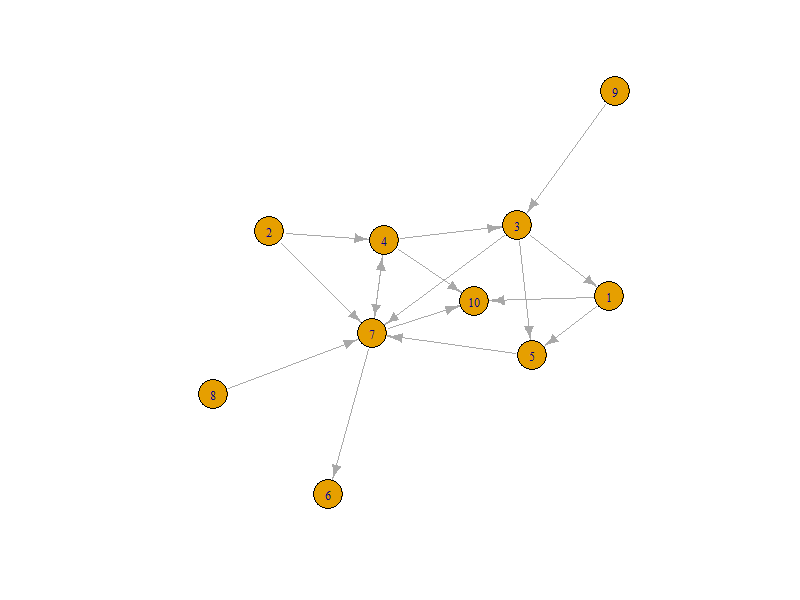
\includegraphics[height=11cm]{partials/images/graph_directed.png}
	\caption{Przykład grafu skierowanego}
\label{Fig:GraphUndirected}
\end{figure}
\FloatBarrier

Graf nieskierowany to graf, w którym krawędzie nie mają kierunku.
Możemy mieć tylko jedną krawędź łączącą dwa wierzchołki (ponieważ V to zbiór).
Zwykle pętle w wierzchołkach nie są pożądane.
Wszystkie grafy są nieskierowane, chyba że zaznaczono inaczej.

\begin{figure}[ht]
	\centering
	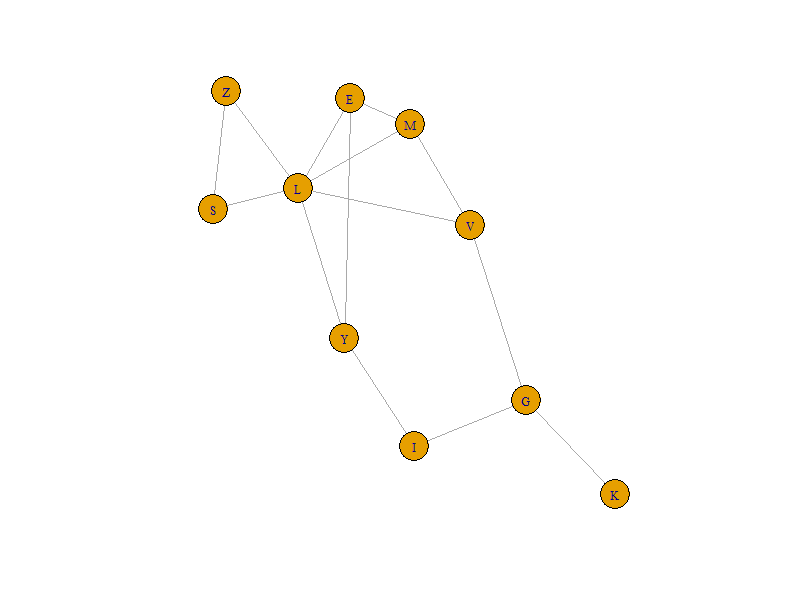
\includegraphics[height=11cm]{partials/images/graph_undirected.png}
	\caption{Przykład grafu nieskierowanego}
    \label{Fig:GraphDirected}
\end{figure}
\FloatBarrier

\subsection{Rozpoznawanie grafów}
Lorem Ipsum is simply dummy text of the printing and typesetting industry. Lorem Ipsum has been the industry's standard dummy text ever since the 1500s, when an unknown printer took a galley of type and scrambled it to make a type specimen book. It has survived not only five centuries, but also the leap into electronic typesetting, remaining essentially unchanged. It was popularised in the 1960s with the release of Letraset sheets containing Lorem Ipsum passages, and more recently with desktop publishing software like Aldus PageMaker including versions of Lorem Ipsum.
